\documentclass[11pt]{article}
\usepackage[margin=0.78in]{geometry}
\usepackage{amsmath,amssymb,booktabs,longtable,graphicx,xcolor,array,seqsplit,float}
\usepackage[hidelinks]{hyperref}
\newcommand{\dt}{\Delta t}
\newcommand{\ii}{\mathrm{i}}
\newcommand{\pass}{\textcolor{green!45!black}{PASS}}
\newcommand{\fail}{\textcolor{red!75!black}{FAIL}}
\title{Targeted EDMD Completeness Test for the Three-Mode Oscillatory Mode}
\author{Analysis-only numerical audit}
\date{7 September 2026}

\begin{document}
\maketitle

\begin{abstract}
The predeclared raw-action/cross-term extension exposes a complex EDMD
candidate with imaginary part near the independently measured frequency
$5.1$--$5.5$. Three of four bath/timestep cases pass every frozen candidate
gate, but the driven $\dt=10^{-3}$ case fails dictionary convergence: at
$\tau=0.05$, E1, E2 and E3 give real parts $-6.466,-5.112,-5.520$, whose
range $1.354$ exceeds the frozen tolerance $1.104$. Consequently the requested
four-case completeness test \emph{fails}; the EDMD spectrum remains incomplete.
The extension also moves the slowest visible real rate from approximately
$-0.95$ to approximately $-0.90$--$-0.92$ (non-overlapping old/new confidence
intervals in three of four cases). Thus the old $-0.95$ value was
dictionary-sensitive and cannot be promoted to the slowest rate of the full
generator spectrum.
\end{abstract}

\section{Frozen question and interpretation gate}

This is not a new stochastic simulation. It reuses the four controlled
$n=3$ trajectory ensembles (64 independent streams, burn-in 500, stationary
time 1000, snapshots every 0.01) from the double-precision, fixed-timestep,
standard-trigonometry, projection-free implementation. The protocol was
frozen in commit \texttt{0af6652} before any extended spectrum was computed.

The original D1/D2/D3 log-action--Fourier bases were augmented once with the
same 19 predeclared raw features: $I_1,I_2,I_3$, their six quadratic products,
and the ten requested functions built from $dI=I_1-I_3$, including
$dI\cos\theta_1$, $dI\sin\theta_1$, $dI\cos\theta_3$,
$dI\sin\theta_3$, $dI\cos(\theta_1-\theta_3)$ and
$dI\sin(\theta_1-\theta_3)$. The nominal sizes are E1/E2/E3=
109/269/519. No function was added after looking at the spectra.

The frozen interpretation was: recover the oscillation and leave the leading
real confidence interval unchanged to promote the slow rate; recover it but
move the rate to diagnose the old rate as dictionary-limited; otherwise declare
the spectrum incomplete. The last branch applies.

\section{Primary result: targeted oscillatory mode}

The reference in each case was chosen deterministically from E3 at
$\tau=0.05$: $4.5\leq\Im\lambda\leq6$, $-20\leq\Re\lambda\leq-0.05$,
then largest real part. Bootstrap intervals resample the 64 complete
trajectories 500 times.

\begin{table}[H]
\centering\small
\caption{Primary complex candidate. ``AC'' is the independent damped-
oscillation estimate from $I_1-I_3$. Intervals are trajectory-bootstrap 95\%
intervals.}
\begin{tabular}{@{}lrrrrrrc@{}}
\toprule
case & $\Re\lambda$ & 95\% CI & $\Im\lambda$ & 95\% CI & AC $\Im\lambda$ & accepted & gate\\
\midrule
driven, $10^{-3}$ & $-5.520$ & $[-6.027,-4.885]$ & $5.037$ & $[4.467,5.674]$ & $5.401$ & 500/500 & \fail\\
driven, $2.5\,10^{-4}$ & $-5.582$ & $[-6.132,-4.828]$ & $5.696$ & $[5.077,6.302]$ & $5.500$ & 500/500 & \pass\\
equal, $10^{-3}$ & $-5.060$ & $[-5.877,-4.750]$ & $5.831$ & $[5.112,6.339]$ & $5.081$ & 500/500 & \pass\\
equal, $2.5\,10^{-4}$ & $-5.963$ & $[-6.297,-5.403]$ & $5.293$ & $[4.778,5.776]$ & $5.264$ & 500/500 & \pass\\
\bottomrule
\end{tabular}
\end{table}

The independent frequency lies inside three EDMD intervals. In the equal
$10^{-3}$ case it lies just below the EDMD lower endpoint (by 0.031), while the
point estimates differ by 0.750. Therefore even the frequency comparison is
not a four-case agreement. The EDMD real parts agree with the independently
fitted driven damping rates ($-5.024,-5.003$) within their broad EDMD intervals,
but not with the equal-temperature damping rates ($-4.141,-4.184$). This is
additional evidence that the selected equal-temperature candidates should not
be identified as the complete known mode without qualification.

\subsection{Dictionary gate}

\begin{table}[H]
\centering\small
\caption{Matched candidates at $\tau=0.05$, shown as
$\Re\lambda+\ii\Im\lambda$. Only the first row violates the predeclared
20\% stability rule.}
\begin{tabular}{@{}lcccc@{}}
\toprule
case & E1 & E2 & E3 & gate\\
\midrule
driven, $10^{-3}$ & $-6.466+4.904\ii$ & $-5.112+4.918\ii$ & $-5.520+5.037\ii$ & \fail\\
driven, $2.5\,10^{-4}$ & $-5.404+6.194\ii$ & $-5.698+5.066\ii$ & $-5.582+5.696\ii$ & \pass\\
equal, $10^{-3}$ & $-5.010+5.464\ii$ & $-5.768+5.315\ii$ & $-5.060+5.831\ii$ & \pass\\
equal, $2.5\,10^{-4}$ & $-5.476+5.692\ii$ & $-5.736+5.416\ii$ & $-5.963+5.293\ii$ & \pass\\
\bottomrule
\end{tabular}
\end{table}

For the failed row, the real-part range is 1.3536 versus tolerance 1.1039;
the imaginary-part range is 0.1329 versus tolerance 0.9836. Thus it is the
damping estimate, not the frequency, that fails dictionary convergence.
Retained/nominal Gram dimensions (E1,E2,E3) were respectively
107/109, 267/269, 517/519; 106/109, 266/269, 516/519; 107/109,
267/269, 516/519; and 107/109, 267/269, 517/519 in table order.

\begin{figure}[H]
\centering
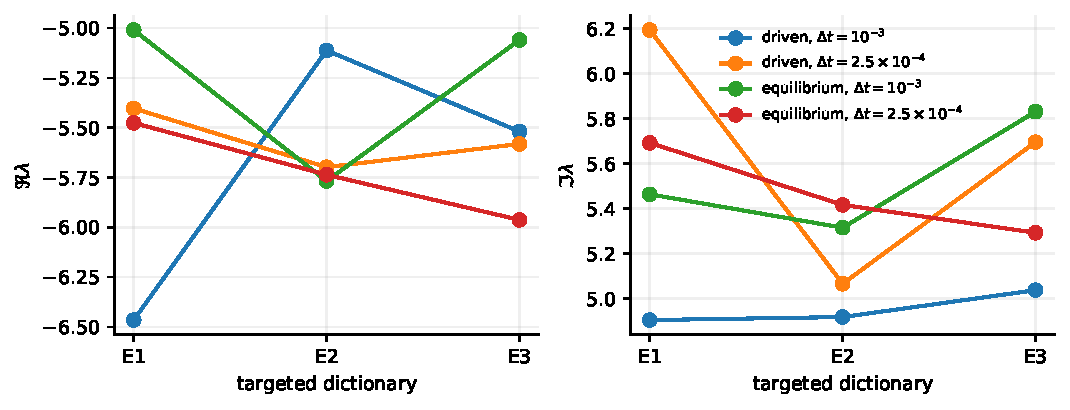
\includegraphics[width=.92\linewidth]{../figures/oscillatory_dictionary_convergence.pdf}
\caption{Dictionary dependence at the predeclared reference lag.}
\end{figure}

\subsection{Short- and long-lag checks}

All three short lags are far below their principal-log Nyquist bounds and pass
the frozen lag-spread gate. The exact matched values are:

\begin{table}[H]
\centering\scriptsize
\caption{E3 short-lag candidates. Nyquist bounds for $\tau=0.02,0.05,0.10$
are 157.080, 62.832 and 31.416, respectively; none is aliased.}
\begin{tabular}{@{}lccc@{}}
\toprule
case & $\tau=.02$ & $\tau=.05$ & $\tau=.10$\\
\midrule
driven, $10^{-3}$ & $-5.673+5.271\ii$ & $-5.520+5.037\ii$ & $-5.307+5.305\ii$\\
driven, $2.5\,10^{-4}$ & $-5.194+5.709\ii$ & $-5.582+5.696\ii$ & $-5.296+5.409\ii$\\
equal, $10^{-3}$ & $-5.252+5.609\ii$ & $-5.060+5.831\ii$ & $-4.410+6.500\ii$\\
equal, $2.5\,10^{-4}$ & $-5.602+5.294\ii$ & $-5.963+5.293\ii$ & $-5.913+5.008\ii$\\
\bottomrule
\end{tabular}
\end{table}

\begin{figure}[H]
\centering
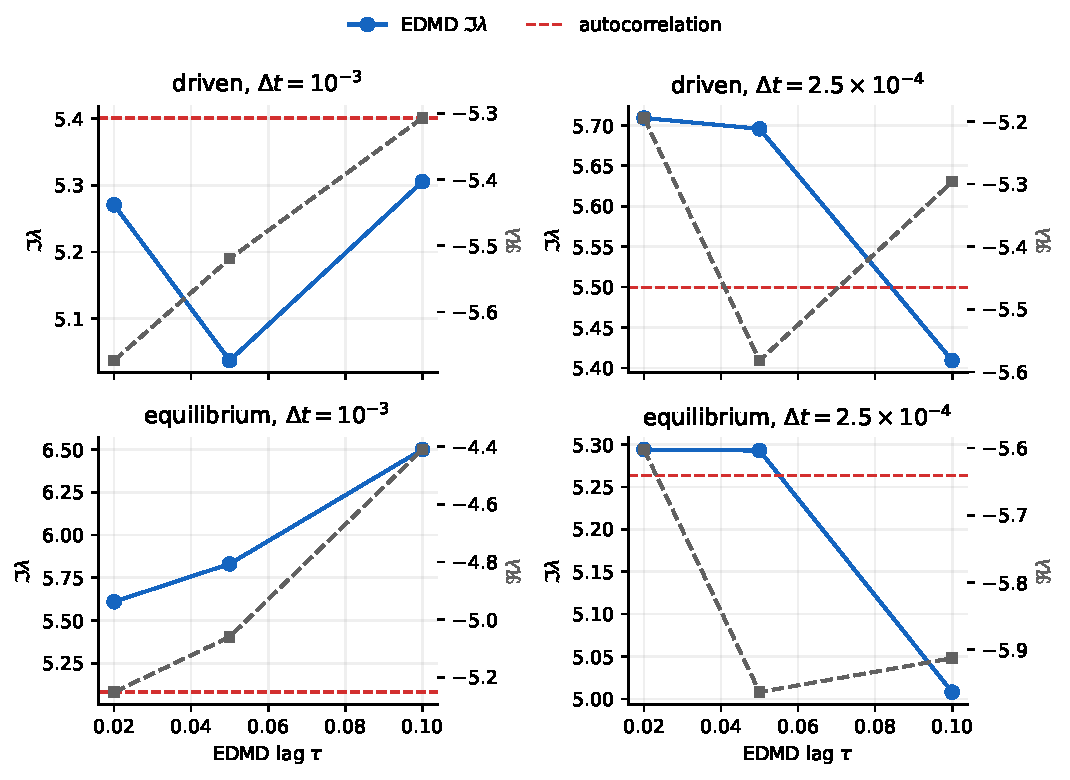
\includegraphics[width=.92\linewidth]{../figures/oscillatory_short_lag_convergence.pdf}
\caption{Short-lag convergence. Blue is the matched EDMD frequency; red is
the independently fitted $I_1-I_3$ frequency. Grey, on the right axes, is the
EDMD real part.}
\end{figure}

Long lags provide the predicted aliasing diagnostic rather than evidence for
convergence. At $\tau=0.25$ (Nyquist 12.566), no row is aliased. At
$\tau=0.50$ (Nyquist 6.283; 20\% exclusion threshold 5.027), three of four
rows are aliased; only driven $10^{-3}$, with $\Im\lambda=4.951$, remains just
outside the exclusion region. At $\tau=1$ all four matches sit exactly at
$\Im\lambda=\pi$ and are marked aliased. The long-lag values are retained in
\texttt{oscillatory\_convergence.csv}; they do not enter the short-lag gate.

The cutoff check is numerically flat to the printed precision at
$10^{-8},10^{-10},10^{-12}$ in every case. At E3/$\tau=.05$, the primary
Gram condition numbers range from $6.41\,10^8$ to $6.38\,10^9$; the truncated
$10^{-8}$ fits retain 515 directions and have condition numbers
$2.19\,10^5$--$3.25\,10^5$, yet produce the same target eigenvalues. Every
constant-mode error is below $1.28\,10^{-12}$ (required $10^{-8}$).

\section{Leading visible real mode}

The targeted extension changes the leading visible real mode. Each new row
passes dictionary, original-lag, timestep, cutoff, 500-bootstrap and neighbour
separation gates, but ``reportable'' here means only within the tested EDMD
subspaces, not proven leading in the full spectrum.

\begin{table}[H]
\centering\small
\caption{Original and enlarged-dictionary leading visible real rates.}
\begin{tabular}{@{}lrrrrc@{}}
\toprule
case & old & old 95\% CI & new & new 95\% CI & disjoint?\\
\midrule
driven, $10^{-3}$ & $-0.9402$ & $[-0.9546,-0.9208]$ & $-0.8998$ & $[-0.9164,-0.8826]$ & yes\\
driven, $2.5\,10^{-4}$ & $-0.9632$ & $[-0.9800,-0.9419]$ & $-0.9224$ & $[-0.9435,-0.9024]$ & no (marginal)\\
equal, $10^{-3}$ & $-0.9551$ & $[-0.9724,-0.9328]$ & $-0.9058$ & $[-0.9227,-0.8886]$ & yes\\
equal, $2.5\,10^{-4}$ & $-0.9408$ & $[-0.9548,-0.9230]$ & $-0.8945$ & $[-0.9118,-0.8777]$ & yes\\
\bottomrule
\end{tabular}
\end{table}

\begin{figure}[H]
\centering
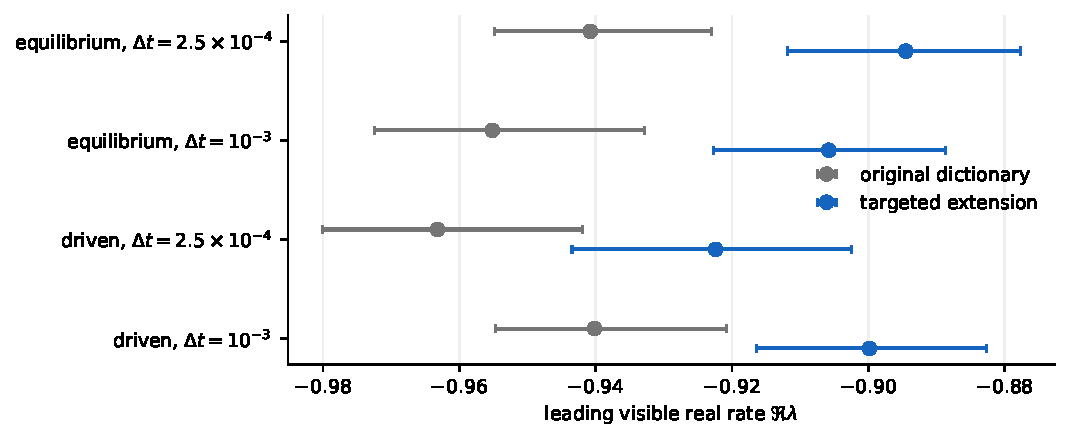
\includegraphics[width=.9\linewidth]{../figures/leading_real_old_vs_extended.pdf}
\caption{The extension shifts all four leading visible point estimates toward
zero. Three old/new interval pairs are disjoint.}
\end{figure}

The two driven timesteps now give $-0.9003$ and $-0.9227$; the two equilibrium
timesteps give $-0.9055$ and $-0.8942$. The rate is therefore stable near
$-0.91$ within the enlarged dictionary, but the movement establishes that the
old $-0.95$ estimate was dictionary-limited. Because the oscillatory
completeness gate fails, $-0.91$ is still only the slowest mode visible to E1--E3.

The two driven candidates near $-1.8$ and $-2.1$ do not separate. Their
bootstrap intervals are $[-1.900,-1.558]$ and $[-2.159,-1.786]$ at
$\dt=10^{-3}$, and $[-1.882,-1.677]$ and $[-2.160,-1.789]$ at
$\dt=2.5\,10^{-4}$; both pairs overlap. This secondary test fails.

\section{Updated modal weights}

\begin{table}[H]
\centering\small
\caption{Absolute covariance weights on the new leading visible mode.}
\begin{tabular}{@{}lrrrr@{}}
\toprule
case & $I_2$ & $I_1+I_3$ & $\cos\theta_3$ & cosine sum\\
\midrule
driven, $10^{-3}$ & .492 & .294 & .121 & .214\\
driven, $2.5\,10^{-4}$ & .485 & .285 & .122 & .218\\
equal, $10^{-3}$ & .470 & .268 & .103 & .203\\
equal, $2.5\,10^{-4}$ & .466 & .270 & .101 & .202\\
\bottomrule
\end{tabular}
\end{table}

The robust ordering $I_2>I_1+I_3$ survives and remains consistent with their
controlled autocorrelation plateaus $-0.935$ and $-1.003$. The strict
monotone correspondence does \emph{not} survive for the two cosine observables:
the cosine-sum weight is larger than the $\cos\theta_3$ weight, while their
plateaus are $-1.122$ and $-1.092$, respectively. Modal weight alone therefore
does not totally order the finite-window autocorrelation fits.

\begin{figure}[H]
\centering
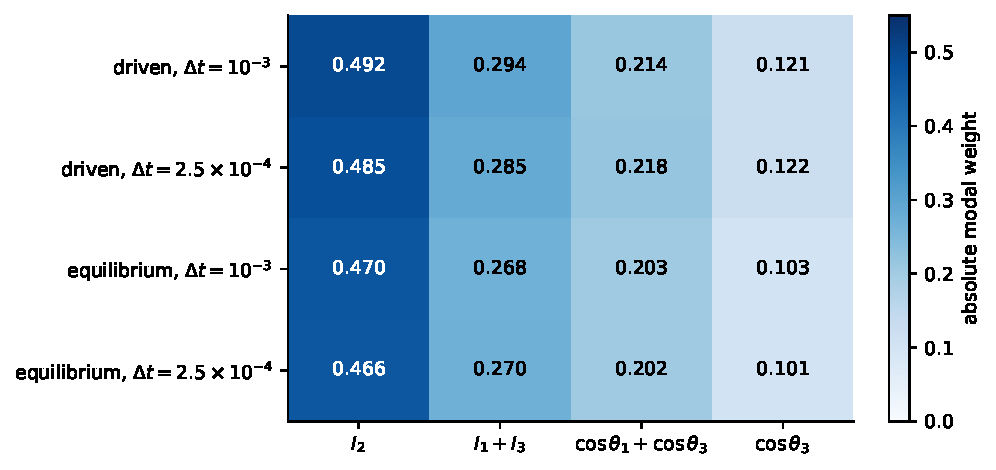
\includegraphics[width=.82\linewidth]{../figures/leading_modal_weights.pdf}
\caption{Leading-mode covariance weights after the dictionary extension.}
\end{figure}

\section{Eigenfunction slices}

The requested equal-action slices were computed at $I_1=I_2=I_3=1,2,4$ for
both the selected oscillatory candidate and the leading visible real mode in
all four cases. Figure~\ref{fig:slices} shows one representative case. Since
the overall oscillatory gate fails, the upper row is a diagnostic candidate
eigenfunction, not a validated generator eigenfunction. All four raw slice
tables and figures are included in the package.

\begin{figure}[H]
\centering
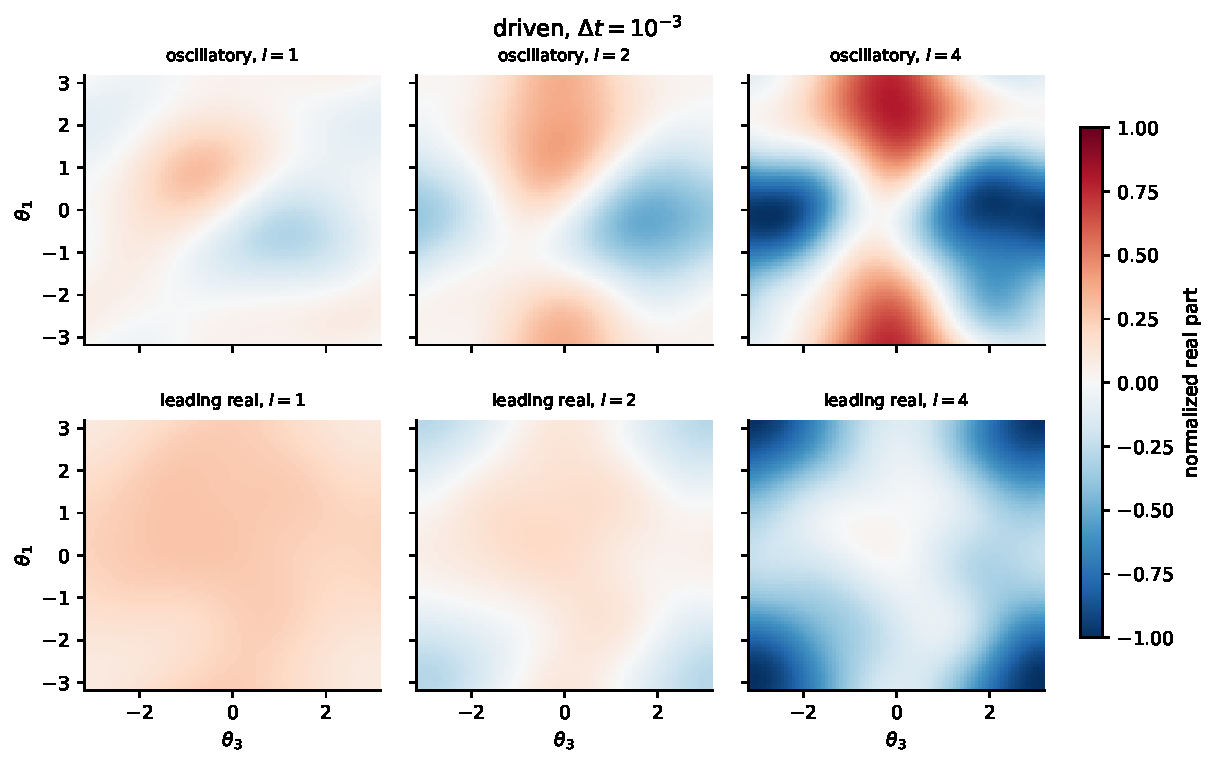
\includegraphics[width=.62\linewidth]{../figures/driven_dt1e-3_eigenfunction_slices.pdf}
\caption{Normalized real parts of the two EDMD eigenfunctions for the driven
$\dt=10^{-3}$ case.}\label{fig:slices}
\end{figure}

\section{Provenance and reproducibility}

The analysis source was frozen in commit \texttt{70cbab9}; its SHA-256 is
\texttt{\seqsplit{a986b0cc1d3f0e190223d348d7522b2ac81ce307e0628fd00852b2329aee2c57}}.
The imported original EDMD helper has SHA-256
\texttt{\seqsplit{d4c53270ed902cbcf6692dcc64d7c1f423e40189504d03703c6e4f8cd50cc6ef}}.
The controlled trajectory simulator source and binary hashes are respectively
\texttt{\seqsplit{58c871882f1180701a7aae637a8f4be113315a72fb9d7815562f5fc90faf7976}}
and \texttt{\seqsplit{f7cd820bb8f716a8790f688db060259da5657e4f20fa09100546e66efb696b3f}}.
Base stream seeds were 2026090801--2026090804 by case; each generated 64
independent stream seeds according to the saved controlled-run manifest.
Bootstrap base seed was 2026090702, offset by case; real-mode bootstrap used an
additional offset 100.

The exact analysis command was:
\begin{verbatim}
python3 experiments/edmd_oscillatory_extension_2026-09-07/
  run_extended_edmd.py \
  --input experiments/spectral_gap_controlled_2026-09-07/raw \
  --output experiments/edmd_oscillatory_extension_2026-09-07/analysis
\end{verbatim}
followed by the frozen gate command:
\begin{verbatim}
python3 experiments/edmd_oscillatory_extension_2026-09-07/
  summarize_extended_edmd.py \
  --analysis experiments/edmd_oscillatory_extension_2026-09-07/analysis
\end{verbatim}

The integrity audit found 256/256 input streams with the expected size,
all four aggregate matrices with expected dimensions, 500/500 oscillatory
bootstrap rows per case, 500 rows per tracked real mode, finite spectra, and
all constant-mode checks passing. Full input and output SHA-256 manifests are
in \texttt{provenance/}. The raw spectra, all per-replicate bootstrap fits,
convergence tables, aggregate EDMD matrices, weights and eigenfunction slices
are included rather than replaced by this report.

\section{Claim boundary}

The targeted extension substantially improves visibility of the known
oscillatory frequency, but it does not pass the predeclared four-case
dictionary-completeness test. The defensible statement is:
\begin{quote}
The enlarged raw-action EDMD dictionary reveals a reproducible complex
candidate near the independently observed oscillation and a stable slow
visible rate near $-0.91$, but one dictionary gate fails and the slow rate moves
relative to the original basis. Hence the complete generator spectrum and its
spectral gap remain unresolved.
\end{quote}
No additional basis was tested in this task.

\end{document}
